% This is "sig-alternate.tex" V2.0 May 2012
% This file should be compiled with V2.5 of "sig-alternate.cls" May 2012
%
% This example file demonstrates the use of the 'sig-alternate.cls'
% V2.5 LaTeX2e document class file. It is for those submitting
% articles to ACM Conference Proceedings WHO DO NOT WISH TO
% STRICTLY ADHERE TO THE SIGS (PUBS-BOARD-ENDORSED) STYLE.
% The 'sig-alternate.cls' file will produce a similar-looking,
% albeit, 'tighter' paper resulting in, invariably, fewer pages.
%
% ----------------------------------------------------------------------------------------------------------------
% This .tex file (and associated .cls V2.5) produces:
%       1) The Permission Statement
%       2) The Conference (location) Info information
%       3) The Copyright Line with ACM data
%       4) NO page numbers
%
% as against the acm_proc_article-sp.cls file which
% DOES NOT produce 1) thru' 3) above.
%
% Using 'sig-alternate.cls' you have control, however, from within
% the source .tex file, over both the CopyrightYear
% (defaulted to 200X) and the ACM Copyright Data
% (defaulted to X-XXXXX-XX-X/XX/XX).
% e.g.
% \CopyrightYear{2007} will cause 2007 to appear in the copyright line.
% \crdata{0-12345-67-8/90/12} will cause 0-12345-67-8/90/12 to appear in the copyright line.
%
% ---------------------------------------------------------------------------------------------------------------
% This .tex source is an example which *does* use
% the .bib file (from which the .bbl file % is produced).
% REMEMBER HOWEVER: After having produced the .bbl file,
% and prior to final submission, you *NEED* to 'insert'
% your .bbl file into your source .tex file so as to provide
% ONE 'self-contained' source file.
%
% ================= IF YOU HAVE QUESTIONS =======================
% Questions regarding the SIGS styles, SIGS policies and
% procedures, Conferences etc. should be sent to
% Adrienne Griscti (griscti@acm.org)
%
% Technical questions _only_ to
% Gerald Murray (murray@hq.acm.org)
% ===============================================================
%
% For tracking purposes - this is V2.0 - May 2012

\documentclass{sig-alternate-nocopyright}

\usepackage{url}
\usepackage{hyperref}
\begin{document}
%
% --- Author Metadata here ---
\conferenceinfo{WOODSTOCK}{'97 El Paso, Texas USA}
%\CopyrightYear{2007} % Allows default copyright year (20XX) to be over-ridden - IF NEED BE.
%\crdata{0-12345-67-8/90/01}  % Allows default copyright data (0-89791-88-6/97/05) to be over-ridden - IF NEED BE.
% --- End of Author Metadata ---

\subtitle{CMU 18-749 Fall 2015 Class Project}
\title{Biometer: Fault Tolerant Healthcare Aggregator}
%
% You need the command \numberofauthors to handle the 'placement
% and alignment' of the authors beneath the title.
%
% For aesthetic reasons, we recommend 'three authors at a time'
% i.e. three 'name/affiliation blocks' be placed beneath the title.
%
% NOTE: You are NOT restricted in how many 'rows' of
% "name/affiliations" may appear. We just ask that you restrict
% the number of 'columns' to three.
%
% Because of the available 'opening page real-estate'
% we ask you to refrain from putting more than six authors
% (two rows with three columns) beneath the article title.
% More than six makes the first-page appear very cluttered indeed.
%
% Use the \alignauthor commands to handle the names
% and affiliations for an 'aesthetic maximum' of six authors.
% Add names, affiliations, addresses for
% the seventh etc. author(s) as the argument for the
% \additionalauthors command.
% These 'additional authors' will be output/set for you
% without further effort on your part as the last section in
% the body of your article BEFORE References or any Appendices.

\numberofauthors{3} %  in this sample file, there are a *total*
% of EIGHT authors. SIX appear on the 'first-page' (for formatting
% reasons) and the remaining two appear in the \additionalauthors section.
%
\author{
% You can go ahead and credit any number of authors here,
% e.g. one 'row of three' or two rows (consisting of one row of three
% and a second row of one, two or three).
%
% The command \alignauthor (no curly braces needed) should
% precede each author name, affiliation/snail-mail address and
% e-mail address. Additionally, tag each line of
% affiliation/address with \affaddr, and tag the
% e-mail address with \email.
%
% 1st. author
\alignauthor
Mikhail Kutsovsky\\
       \affaddr{Dept. of Electrical \& Computer Engineering}\\
       \affaddr{Carnegie Mellon University}\\
       \affaddr{Pittsburgh, PA, USA}\\
       \email{mkutsovs@andrew.cmu.edu}
% 2nd. author
\alignauthor
Joshua Antonson\\
       \affaddr{Dept. of Electrical \& Computer Engineering}\\
       \affaddr{Carnegie Mellon University}\\
       \affaddr{Pittsburgh, PA, USA}\\
       \email{jantonso@andrew.cmu.edu}
\alignauthor
Aayush Agarwal\\
       \affaddr{Dept. of Electrical \& Computer Engineering}\\
       \affaddr{Carnegie Mellon University}\\
       \affaddr{Pittsburgh, PA, USA}\\
       \email{aayusha@andrew.cmu.edu}
}
% There's nothing stopping you putting the seventh, eighth, etc.
% author on the opening page (as the 'third row') but we ask,
% for aesthetic reasons that you place these 'additional authors'
% in the \additional authors block, viz.
% Just remember to make sure that the TOTAL number of authors
% is the number that will appear on the first page PLUS the
% number that will appear in the \additionalauthors section.

\maketitle
\begin{abstract}
As individuals get older and spend time in various places around the country, the necessity to visit different doctors, for different ailments all located in different locations becomes an inevitability. Each visit leaves a fragment of that individuals health record behind, often times to never to be seen again. The  medical records and other relevant information accessible to patients used in electronic personal health record systems (PHRs), which are the cornerstones of patient centered healthcare, are incomplete (in a possibly critical fashion) due to this fragmentation and cannot optimally assist patients through health self-management. This paper proposes a solution to the difficulty of gathering this fragmented information through an automated scraping process that gathers information from various sources in one place. This  compiled medical history can be leveraged to provide greater benefits than any stand-alone systems due to the completeness of the information.
\end{abstract}

% A category with the (minimum) three required fields
\category{H.4}{Information Systems Applications}{Miscellaneous}

\terms{}
Personal Health Record. Fault Tolerant Distributed System. Web Scraping. Databases. User Experience
%\keywords{}

\section{Introduction}
The trend of hospitals and medical providers moving towards electronic medical records as well as the prevalent use and availability of medical information online is setting up a situation where patients have a lot more control over their health care and treatment. Studies have shows that 42 percent of the US population keeps records for themselves, 87 percent of these being in paper format\cite{taylor2004} and that doing this is a very good idea. Many trials of electronic personal health record systems (PHRs) have shown that they supplement and improve patient and family access to knowledge for self-management of health and wellness issues \cite{jones2010}. With all of these clear benefits to having PHRs and multiple initiatives from medical providers to offer Personal Health Record systems  with their care how come it is still so difficult for the general population to get access to their documents from various providers and ensure that all the doctors they see have a unified view of their health situation. We take the approach that a PHR that is based on the provider giving the information as opposed to the patient seeking out the information is inherently flaws. Due to the variety of websites, incompatibility of PHR systems across providers and the large amount of health information which will not be accessible in this manner, relying on the provid. Since we cannot rely on providers to have all the information needed for a complete medical history available in a easily accessible manner, we have built Biometer to be a fault-tolerant application which can perform scraping operations against various medical providers on behalf of the user. The capability of going out and proactively reaching out to all the medical providers an individual has had contact with will result in a much more comprehensive medical record that will benefit care in every aspect.

\section{Problem Statement}
Collecting information from hospitals and medical providers is an unexpectedly difficult task for a person to do. Jumping through the various process requirements of these institutions before actually getting ones information is a major deterrent for people. To fix this problem we need to build a system that can automatically and reliably get the desired medical records with minimal input from users. The manners in which we can get user medical records from a providers is A) User already has and uploads B) Automated Scraping of the providers patient portal C)Sending Authorization Forms. This system also needs to continue operating under faults and allow user's uninterrupted access and use of this information.
\subsection{Goals}
\begin{enumerate}
\item{Usability: Development of an application where users can create an account, get medical information from supported medical providers via automated web scraping after providing credentials and the capability to then view these records after the fact}
\item{Fault Tolerance: Building a system that is fault tolerant to server's going down in the back-end. Failures should be handled and not effect the user's experience.}
\end{enumerate}
\subsection{Non-goals}
There are a number of issues that need to be addressed before Biometer is ready for public use but they are left for future work. They involve the following:
\begin{enumerate}
\item{We do not aim to support gathering medical records from every hospital or medical provider, just a select few via scraping their patient portal. Further hospitals can be supported by automating the Authorization From process}
\item{Security and Privacy are major issues with many Personal Health Record systems. Topics in which we are not experts and leave that for future work.}
\end{enumerate}

\section{Approach}
We split our work into two major parts: the application which runs the web client and scraping of medical records and the fault tolerance aspect of the system. Careful thought was given to the initial design of Biometer to make it as stateless as possible requiring fault tolerance in a couple key areas.

\subsection{Architecture}
As seen in Figure 1, we built Biometer with a four level architecture using a MEAN stack. Users connect to the application through a \texttt{stateless web portal}. This server runs Passport for authentication connecting to a \texttt{MongoDB} database. After going through the account creation process, users can then elect to add or view information from a hospital. All requests to retrieve information from a medical provider get sent to the \texttt{Master Server} over HTTP. The master server contains the state of the system and coordinates routing to worker servers. The Master Server also keeps track of which worker server's are available and distributes the workload evenly. The \texttt{worker servers} are stateless machines that can be spun up or down based on the current workload. They receive requests to Scrape a particular medical provider's patient portal (with accompanying user credentials) and save the results to the database.
\begin{figure}
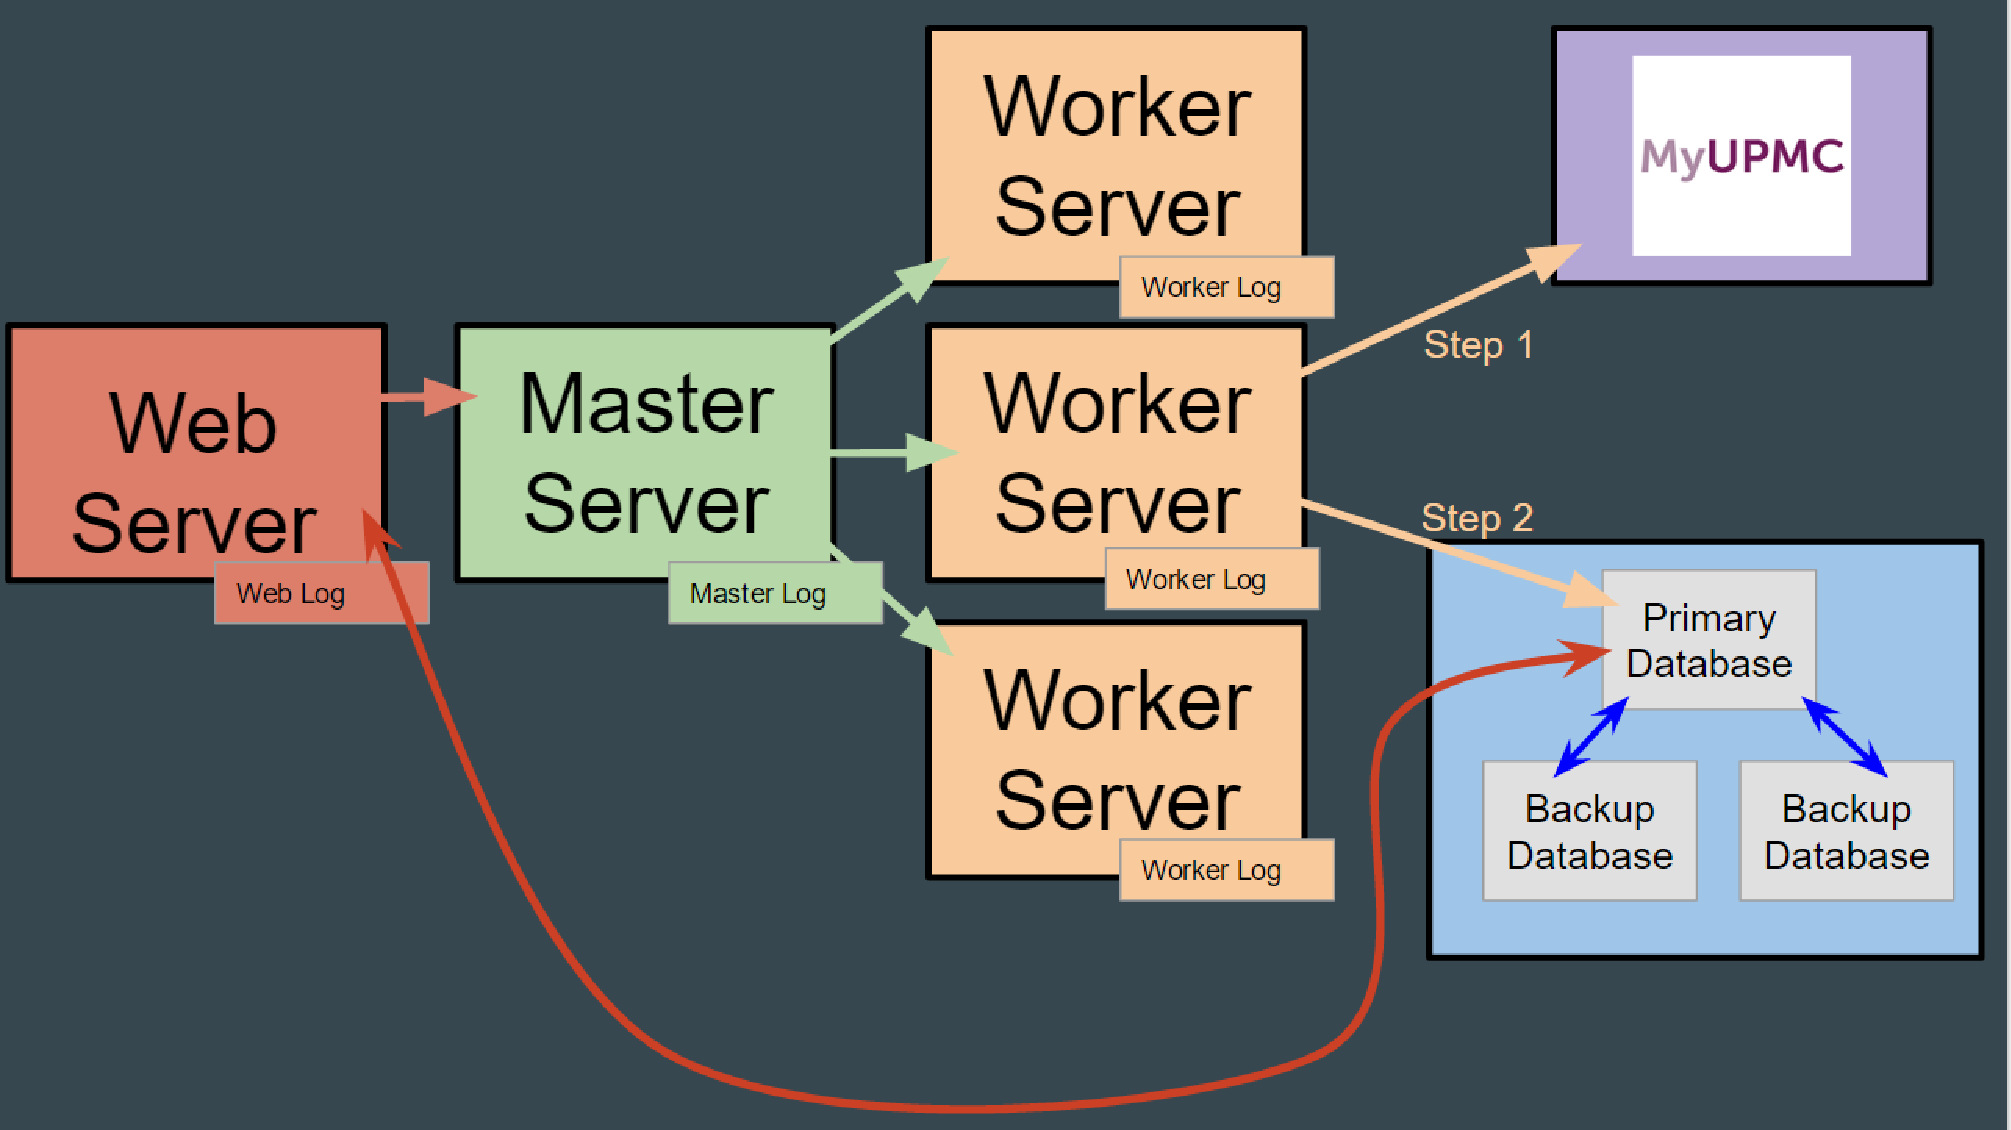
\includegraphics[width=3in]{architecture}
\caption{The Biometer 4-Layer Architecture.}
\end{figure} 
\subsection{Fault Tolerance} 
The Biometer system would ideally have fault tolerance built in at every level of the architecture. The front-end web server contains no state so server crashes here only act as a minor inconvenience to the user. They can just refresh and get connected to a different web server and resume browsing with no loss of data. The Master server is the single point of failure in the application and we would like to passively replicate this server in the future. The Master server is responsible for handling retry logic for any worker server failures. Through the use of asynchronous socket communication between master and worker server, the master is able to immediately detect as a worker goes down, check the list of available workers, and redistribute the incomplete workload to backup worker servers. The MongoDB database is fault tolerant through the use of a primary and secondary replicas. 
\begin{figure}
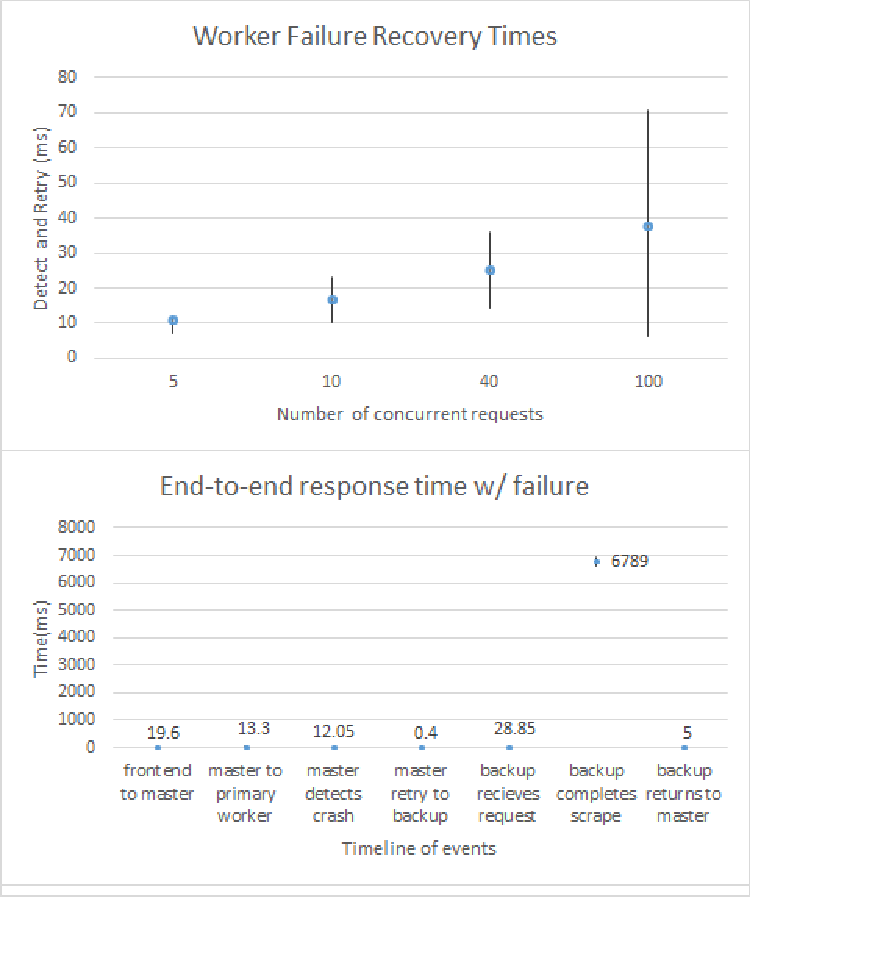
\includegraphics[width=3in]{graphs}
\caption{12ms retry time on worker server failure (top image) and timeline for request w/ retry}
\end{figure}
\section{Experimental Validation}
We analyzed our system through bench marking performance, and recovery times on the University of Pittsburgh Medicine (UPMC) \hyperref[https://myupmc.upmc.com]{patient portal}. We analyzed the system to determine recovery time in the presence of worker faults, as well for execution time of key operations during various workloads.
\subsection{Experimental Setup}
We deployed instances of Front-end, Master and Worker servers as well as our MongoDB instances to AWS on the free tier micro instances. We then simulated various workloads to scrape information from the UPMC account and inserted failures at worker and database layer to monitor the recovery time.
\subsection{Experimental Results}
Due to the use of socket connections to send asynchronous requests from master to worker servers, the fault detection and retry time is ~12ms  and linearly increasing w/ the number of connections open. The time needed to execute a scraping request scales with the number of concurrent requests being serviced by the particular worker with the baseline scrape taking on average 6.5s.
\section{Conclusion}
Biometer is the first step in building a fault tolerant scraping service for medical records. With additional functionality (Authorization Forms, Security and Scale), the approach of taking user credentials and gathering the information on their behalf can enable easy one-click access to a complete medical history.
%
% The following two commands are all you need in the
% initial runs of your .tex file to
% produce the bibliography for the citations in your paper.
\begin{thebibliography}{9}

\bibitem{hillestad05}
  Hillestad, Richard and Bigelow, James and Bower, Anthony and Girosi, Frederico and Meili, Robin and Scobille, Richard and Taylor, Roger,
  \emph{Can Electronic Medical Record Systems Transform Health Care? Potential Health Benefits, Savings, and Costs},
  Health Affairs, 24, no.5 (2005):1103-1117
  
\bibitem{jones2010}
	Jones DA, Shipman JP, Plaut DA, et al.
	\emph{Characteristics of personal health records: findings of the Medical Library Association/National Library of Medicine Joint Electronic Personal Health Record Task Force.}
	 J Med Libr Assoc 2010;98:243–9
	 
\bibitem{taylor2004}
	Taylor H,
	\emph{Two in five adults keep personal or family health records and almost everybody thinks this is a good idea}, 
	Health Care News,
	2004
	
\bibitem{archer2011}
	Archer, N., Fevrier-Thomas, U., Lokker, C., McKibbon, K. A. and Straus, S. E. 
	\emph{Personal health records: a scoping review},
	Journal of the American Medical Informatics Association : JAMIA,
	 18(4), (2011) 515–522. 
\end{thebibliography}
\end{document}
